% --------------------------------------------------
% Capítulo 5: Flood
% --------------------------------------------------
\chapter{Towards Flood-resilient Smart Cities: A Data-driven Risk Assessment Approach Based on Geographical Risks and Emergency Response Infrastructure}\label{cap:flood}
\selectlanguage{english}

\begin{refsection}

\textbf{ABSTRACT}

Flooding in urban areas is expected to become even more common due to climatic changes, putting pressure on cities to implement effective response measures. In fact, practical mechanisms for flood risk assessment have become highly desired, but existing solutions have been devoted to evaluate only particular cities and accounting limited risk perspectives, constraining their applicability in a more generic way. This article presents an innovative approach to assessing the flood risk of delimited urban areas exploiting geospatial information from publicly available databases, providing a method that is applicable to any city in the world requiring minimum configurations. A set of mathematical equations is defined to numerically assess risk levels based on elevation, slope and proximity to rivers, while the existence of emergency-related urban infrastructure is accounted as a risk reduction factor. Then, computed risk levels are used to classify areas, allowing easy visualisation of flood risk over a city. This smart city approach not only serves as a valuable tool for assessing the expected flood risk based on different parameters, but also facilitates the implementation of cutting-edge strategies to effectively mitigate critical situations, ultimately enhancing the urban resilience to flood-related disaster.

\textbf{Keywords:} Emergency evaluation, OpenStreetMap, Risk mitigation, Urban resilience, Sustainability.

\section{Introduction}

Emergencies are not rare events in big cities and metropolises. Actually, because of the fast growing of urban areas and a lack of planning in most of the cities, emergency events are indeed very common~\cite{emergency1,emergency2}. Among the many types of hazardous events, floods are the most recurrent and the one which has most significantly impacted human lives and the cities~\cite{flood,flood2}. Additionally, the current global warming process is believed to cause an increase on the frequency of heavy rains and storms in several cities, putting an additional pressure on urban resilience~\cite{warming,warming_bangladesh}.

%Adicionei
In order to minimise the negative impacts of flooding in cities, different strategies have been adopted lately, ranging from flood risk prediction~\cite{prediction} to rescuing and mitigation response during critical times~\cite{rescuing}. With the advent of sensors to continuously monitor urban areas in real-time, providing information about rainfall index and rivers levels, sensors positioning and communication also became relevant issues~\cite{sensorsposition}. In all these cases, data-driven approaches have emerged as a practical way to better understand the particularities of the target cities and provide the most adequate services in each considered area~\cite{redi}, improving prediction, prevention, and actions during a flooding-related emergency, while also paving the way to the construction of smart cities.

Actually, some researchers have been studying and proposing data-driven methods to assess flood risk in urban areas in order to verify which parts of a city are more prone to suffer from a flooding event~\cite{elevation1,elevation2,elevation3,georeferenced}, potentially demanding better assistance. In such works, specific parameters of each studied city have been usually considered to perform the expected assessment, achieving relevant results. However, besides the usual impossibility to apply a given assessment method to other cities in general, most proposals have been centred on data that are not publicly or easily available for every city, potentially constraining their practical adoption for urban planning and flood-related emergency preparedness. Hence, we consider that open methodologies that make use of publicly available data are of great importance to aid stakeholders and authorities to assess urban risk levels, which should be a guiding development principle in this area~\cite{opendata1,opendata2}.

%Adicionei
Flood risk in urban areas can be directly traced to the geography of a city. First, elevation and slopes are relevant parameters since water will flow to lower regions due to gravity, dictating the flooding behaviour. Second, the existence of rivers within the considered urban area is also a risk since flood may occur when a river reaches its maximum capacity and spills over its banks~\cite{cityflood}. In both cases, the most common causes will be excessive rainfall, rapid snow melting, or even an accident (\textit{e.g}. a dam collapse or a broken pipe), which may be actively measured for the emission of emergency alerts and execution of evacuation actions~\cite{damiot}. Although such measures are valid in many cases, it is usually important to previously identify critical areas that are more prone to flooding: these will be the areas that will need quicker assistance and better rescuing plans. 

%Adicionei
Therefore, when retrieving data from open databases for processing and decision-making, it is possible to better assess urban flood risk, particularly when data from different domains are combined. The idea herein is not to perform flood detection or prediction (which may be performed by other systems), but to estimate how badly an area will be affected by a flood, in average. In this context, flood risk will be assessed in this article based on the combination of relief (expected tendency to accumulate water), rivers crossing urban areas (potential source of flooding), and urban emergency-response infrastructure (capability of a city to quickly respond to a critical situation). While the first two factors account to increasing flood risk in the considered area, the later has an inverse effect, reducing the combined risk perception. Doing so, based on these three data domains, a combined flood risk index will be achieved for every defined urban zone, which might be computed for any city in the world.

This article exploits georeferenced data from OpenStreetMap, a public database with geospatial data collected and configured collaboratively, as well as data from the Open-Elevation API.\ Among the retrieved and computed data, elevation, slope, and distance to rivers are important parameters for flood risk assessment~\cite{elevation1}. Furthermore, data of emergency-response infrastructure will be also retrieved, particularly fire brigades and police stations (for rescuing), and hospitals (to assist victims). 

%Adicionei
To evaluate our proposal, the city of Porto, Portugal, was considered as a case study. The Douro river crossing the city of Porto has an expressive flood history that have made a huge impact in that city more than once, increasing the expected relevance of our approach~\cite{dourohistory}. Figure~\ref{fig:porto_douro} presents a satellite view of that city, highlighting its flooding-prone terrain.

\begin{figure}[ht]
  \centering
  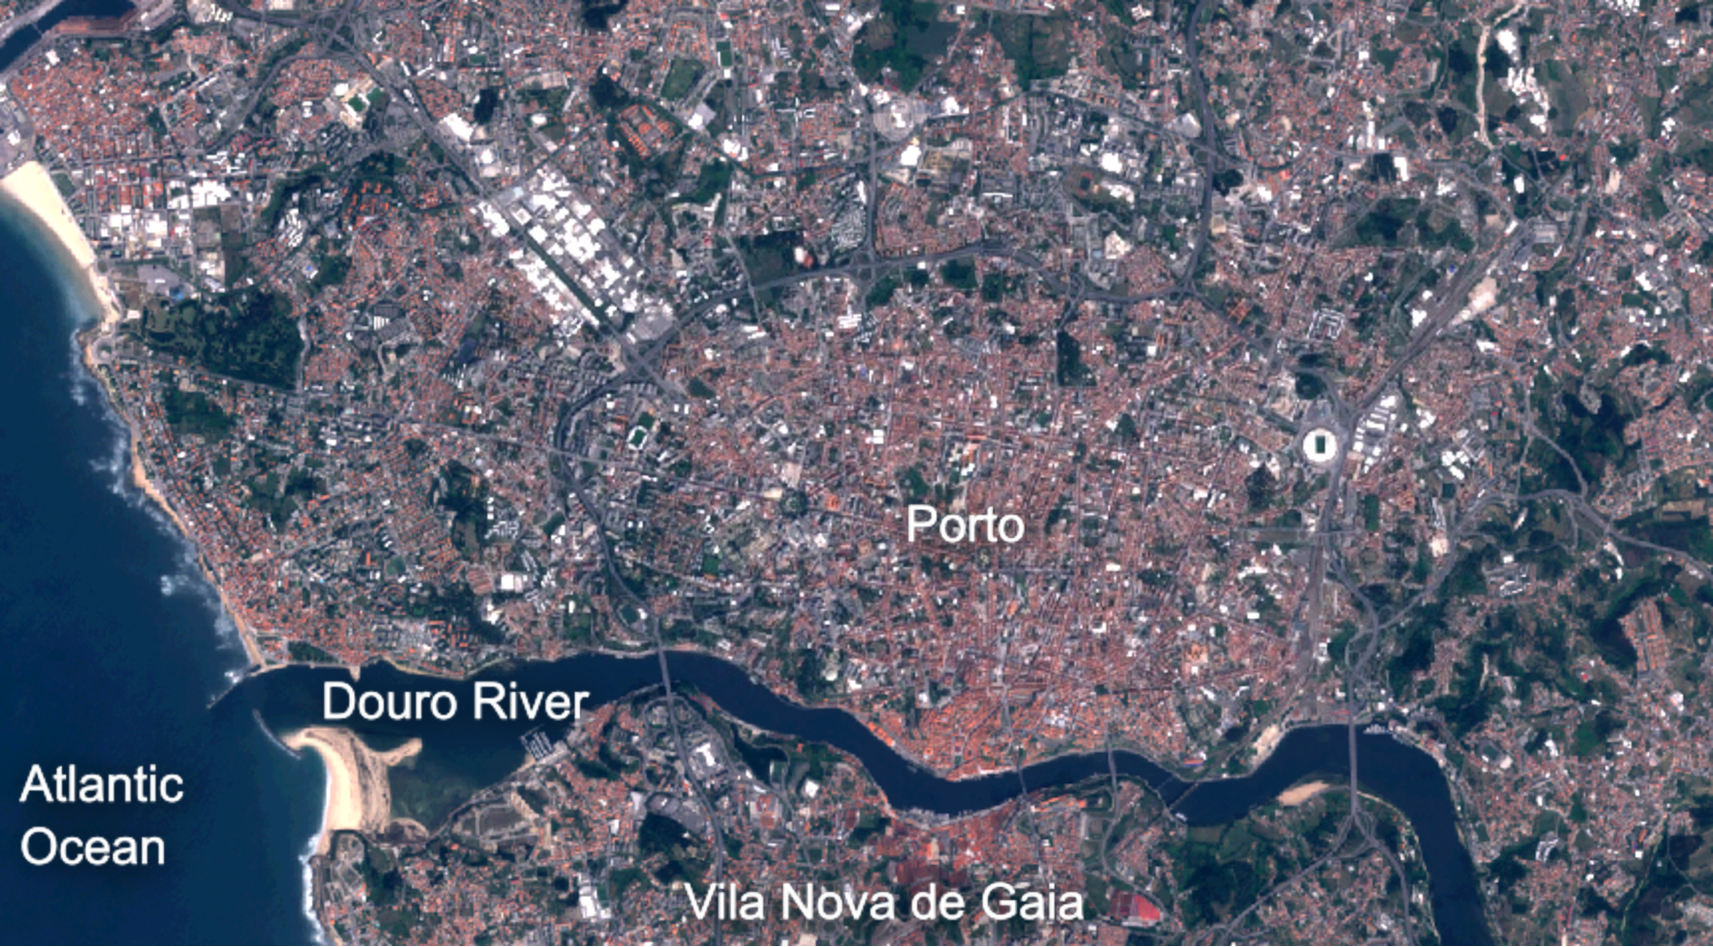
\includegraphics[width=0.9\linewidth]{Chapters/6-Flood/figs/porto_satellite.pdf}
  \caption{A satellite view of the city of Porto, Portugal.}\label{fig:porto_douro}
\end{figure}

The remainder of this article is organised in the following way. Section~\ref{sec:related_works} presents some related works in the area of flood risk assessment. The fundamentals for the intended geospatial data processing are defined in Section~\ref{sec:fundamentals}. Section~\ref{sec:proposal} presents our proposed approach based on a substantial mathematical modelling, while Section~\ref{sec:simulation_ch6} details the performed experiments and the achieved results. Then, Section~\ref{sec:applications} describes potential applications and research trends when exploiting our approach in real scenarios. Finally, conclusions and references are presented.

%%%%%%%%%%%%%%%%%%%%%%%%%%%%%%%%%%%%%%%%%%
\section{Related works}\label{sec:related_works}

Emergency management in smart cities has been studied as a research topic for some years, with several researchers developing methodologies and mathematical models to detect, alert, and mitigate emergency events~\cite{survey,survey2}. When performing such services, the concept of ``urban risk to emergency'' typically associates to the potential threats and vulnerabilities that cities and densely populated areas face regarding the occurrence of emergencies or disasters. Moreover, risk can also be associated to a potential of having negative consequences during critical situations. This way, flood risk will be directly related to excessive water and its urban impacts, with a lot of complexities and variables to be considered, making this a challenging research area~\cite{floodrisk,floodrisk2}.

Emergency risk assessment has been considered as an important element when better creating more resilient cities. Within a smart city scenario, it has been typically assessed based on exposure to critical situations and vulnerability to their negative impacts~\cite{risks1}. In fact, while risk exposure indicates higher probabilities to the occurrence of an emergency, usually due to the physical proximity to a dangerous source (\textit{e.g}. rivers, lakes, and dams), risk vulnerability is an indication of predisposition to be adversely affected by critical events when they happen (lower areas where water may accumulate), which may be associated to elevation and slope. In a different way, urban resilience may be associated to the existence of emergency-response services (\textit{e.g}. fire brigades and rescuing centres), which is a factor that will act to reduce the perceived risk. Although meaningful when processed in a combined way, however, existing literature has been mostly concerned with a single risk perspective, leaving opportunities for improvement.

According to~\cite{flood}, flooding events are the most frequent type of urban emergency, impacting the cities and resulting in economic losses and many other types of damages. Additionally, some studies are linking the global warming with an increase of river floods in several cities~\cite{warming,warming_bangladesh}, which rises an alert on how prone to river floods the big cities will be in the future. In parallel, the negative impacts of heavy rains on cities have also driven many research works~\cite{heavyrain1,heavyrain2}. This way, many works have been concerned with risk assessment based on risk exposure or vulnerability to flooding events.

In order to perform proper risk assessment in a city, regardless of the considered hazard, some of its parameters must be taken in consideration. For example, air humidity is considered in~\cite{fire1} when computing fire risk in some areas, while the work in~\cite{redi} makes use of several parameters (including demographic data) to propose a resilience index for cities. 

In the specific case of flooding there are some particular parameters that must be taken into a risk assessment approach. Initially, it is paramount to define the types of floods that may happen in an urban area: rain flood and river flood~\cite{elevation1}. Regarding rain floods, lower areas with higher zones in its surroundings are more prone to flooding. Also, high slope zones permit the water to flow to lower zones and are less prone to flood in the event of a heavy rain. Regarding river flood, the proximity to the river has a considerable impact~\cite{chapi2017novel}. All these elements define an important risk perception based on exposure to this type of critical event.

Still considering this kind of risk perception, the work in~\cite{elevation1} makes use of elevation and slope data, among other parameters of the studied region, to classify the flood risk levels for the Eldoret Municipality in Kenya. Their approach was based on Analytical Hierarchy Process (AHP) and Geographic Information Systems (GIS) to perform the assessment and was able to generate risk maps for the region with an error level of less than 8\%. Also, the work in~\cite{elevation2} makes use of elevation and slope, among other parameters, as input to a Fuzzy Support Vector Machine (FSVM) to assess flood risk level in the basin of Prahova river, Romania. The authors affirm that the use of FSVM achieved a good performance compared to other models.

While some works make use of region-specific data for risk exposure and vulnerability assessment, the existence of flood response services may be related to urban infrastructure. In~\cite{sensorsposition}, authors consider the existence of emergency-response infrastructure to compute how vulnerable to urban emergencies each urban area is, in an inverse order. In that work, hospitals, fire brigades, and police stations, are used as reference when computing risk vulnerability, with areas worse served by those facilities being considered as riskier. A similar approach is described in~\cite{cityzones}, which provides a highly reconfigurable and open tool to support this type of analysis.

In order to encompass all risk dimensions, this article adopts two publicly and easily accessible data sources. The first source is the Open-Elevation API that contains data for computation of elevation and slope of the zones to assess both rain-flood risk and river-flood risk. The second one is the OpenStreetMap that contains geolocalisation of rivers, enabling the computation of their distances to support the assessment of river-flood risk. Moreover, OpenStreetMap is also used for risk computation based on urban infrastructure, taking advantage of the CityZones tool~\cite{cityzones}, defining the emergency-response risk. Putting all these together, the contributions in this article were not proposed before, to the best of our knowledge. 


%%%%%%%%%%%%%%%%%%%%%%%%%%%%%%%%%%%%%%%%%%
\section{Fundamental concepts}\label{sec:fundamentals}

The flood risk assessment of any urban area will be based on three general parameters: a) the expected flood risk resulted from heavy rain, b) exposure to flood due to the proximity to rivers, and c) the existing urban flooding-response capability, accounted by the presence and proximity to response centres that may perform some mitigation action. These can provide important data on how risky each zone is, with high practical significance. However, before defining the processing of these parameters, some fundamental definitions are required, as presented in next subsections. 

\subsection{Area of Interest}

To assess an urban area regarding the combined flood risk, its perimeter must be initially delimited. Our model defines a polygon area referred as the Area of Interest (AoI), which is segmented in small zones forming a grid-like structure. These zones are the core element of the proposed assessment process, encompassing the fundamental parameters that will be used as input when computing the final flood risk perception. For that, each zone is defined as squares of fixed size $zl$ and location at $(x_c(z), y_c(z))$ position (centre of the defined square), for $|Z|$ zones and $z \in Z$. The position of each zone is required when calculating the distance of each zone to the modelled elements.

Some of the zones may be positioned on an area covered by a river, being referred as ``river zones''. The set of river zones, denoted by $Z_r$, is a subset of $Z$ and every river zone $r \in Z_r$ has the same attributes as an ordinary zone plus the river's flood quota $q(r)$ (described in next subsection). If there are more than one river in the AoI, each river zone will carry the flood quota of the river it belongs to.

An AoI is a polygon that encompass a region of the city that will be classified. In this sense, an AoI is defined by a set of line segments $S$ that connect pairs of points $P = \{P_0, P_1, ..., P_n\}$ forming a polygon defined by $S = \{P_0P_1, P_1P_2, ..., P_{n-1}P_n, P_nP_0\}$. The set $S$ can be directly defined by a stakeholder or retrieved from GIS (Geographic Information System) data as Shapefiles or GeoJSON files. The work in~\cite{cityzones}, exploited by us to retrieve emergency-response data, implements this function using GeoJSON files containing multi-polygon data to define an AoI, which will be adopted by us as reference in this article. After delimiting an AoI, some zones may be inside or outside of its delimited area, requiring exclusion of the zones outside the AoI from the proposed risk assessment process. In other words, the final grid-like structure of the zones will the one that is entirely covered by the defined polygonal area, excluding the zones that the point $(x_c(z), y_c(z))$ is outside the polygonal area of the AoI.

The Area of Interest must be carefully defined as it will limit the effective area for flood risk assessment. For example, in the assessment of a whole city, a polygon comprising the borders of the city can be defined as an AoI. However, if it is desired the assessment of the risk levels of zones within a more specific region, the AoI should be reduced and limited to the effective target region, improving the significance of the results.

\subsection{Emergency-response infrastructure}

Each emergency-response infrastructure in a city is defined as a Point of Interest (PoI), which is basically defined by its GPS position. The nature of the PoIs is typically standardised so they can be processed in a more generic way, although very helpful during a flooding. In this sense, fire brigades are of great importance to mitigate critical situations and support people in the vicinity of the flooded area, mostly due to their rescuing capability during emergencies. And similar reasoning is adopted for police stations and hospitals, since they will have some role when coordinating rescuing operations and when attending victims.

In a scenario of multiple PoIs, a weight value for each of them may be used to determine their level of importance in the assessment process. For example, fire brigades may be more important than hospitals in the mitigation process, thus, they might have a higher weight. Nevertheless, in order to make this general weighting problem more tractable and flexible to be applied in any city, each PoI may have the same relevance and impact during a flood in the common case, but stakeholders and specialists may define specific weights for them.

A PoI is defined by its GPS position at $(x_c(p), y_c(p))$ for any given Point of Interest $p \in P$, where $P$ is the set of PoIs and $|P|$ is the number of PoIs within the defined AoI~\cite{sensorsposition}.

Figure~\ref{fig:zones_and_pois} depicts the zones within an AoI, highlighting the existence of PoIs. The value of $zl$ defines the size of the zones and will determine the resolution of the grid, \textit{i.e}, the smaller the size of the zone, the higher the number of zones forming the grid. Small values for $zl$ can provide more details in the classification results at a higher computation cost. On the other hand, the bigger the AoI, the greater is the chance to find PoIs.

\begin{figure}[ht]
  \centering
  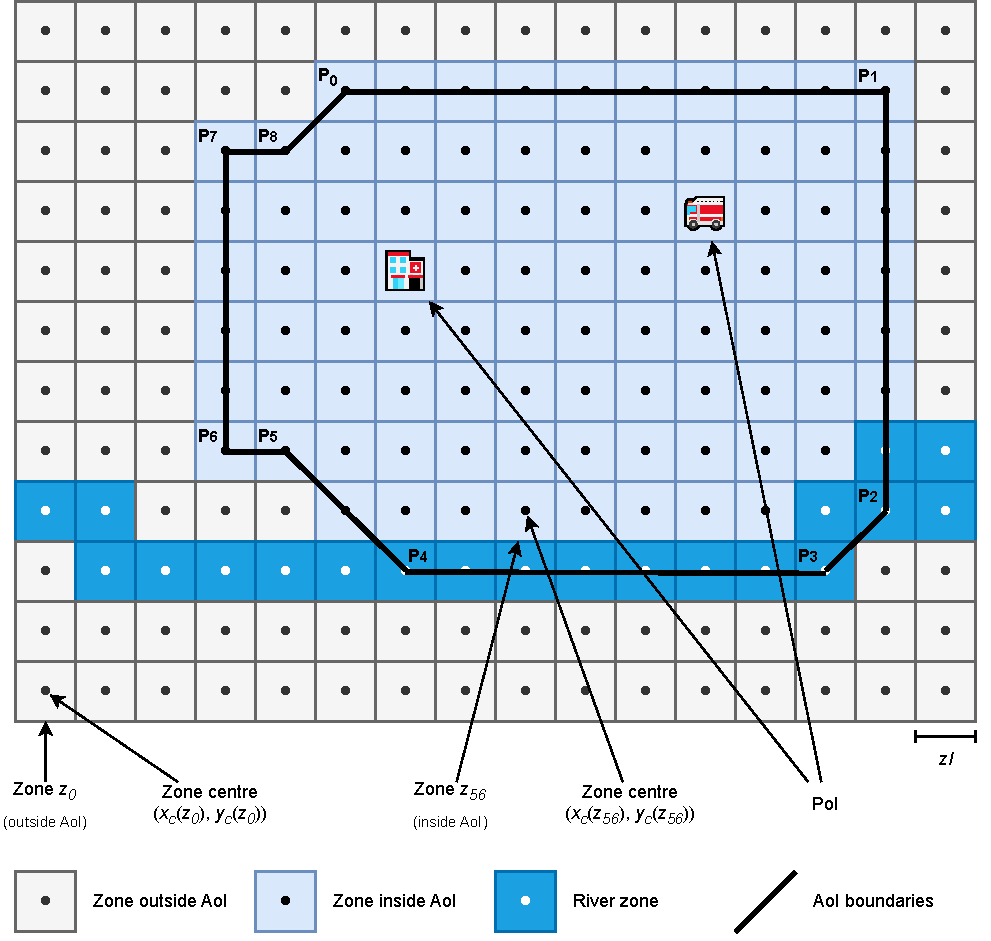
\includegraphics[width=0.9\linewidth]{Chapters/6-Flood/figs/zones_and_pois.pdf}
  \caption{The defined AoI, zones, and PoI modelling.}\label{fig:zones_and_pois}
\end{figure}

%%%%%%%%%%%%%%%%%%%%%%%%%%%%%%%%%%%%%%
\section{Proposed approach}\label{sec:proposal}

Next subsections present the proposed mechanisms to compute the flood parameters (risk perceptions) and the unified flood risk assessment.

%1
\subsection{Elevation data: rain-flood risk}

After the grid has been defined and an AoI has been delimited, the zones can be assessed according to different parameters associated to urban flood. The first considered parameter is related to the zones' relief, since it will impact how water will accumulate during an emergency. 

When computing the flood risk, elevation is a good parameter to assess a general perception of vulnerability, which is, in fact, a measured level of ``susceptibility'' to negative effects in this case~\cite{elevation1,elevation2,elevation3}. From the elevation data of the zones, it is also possible to compute slopes to better perceive such risk. Actually, while lower zones can accumulate water in the event of a heavy rain, water on a high gradient slope terrain flows quickly. The combination of both characteristics will give us a unified perception of how likely a zone will retain water, which is defined by us as the rain-flood risk. 

Figure~\ref{fig:water_flow} shows the typical water flow on a terrain regarding different slopes. Rain water will flow down from high elevation zones, accumulating on lower areas with low gradient slope. Although some areas may be lower than others, if they have a higher gradient slope, water will flow down and will not accumulate.

\begin{figure}[ht]
  \centering
  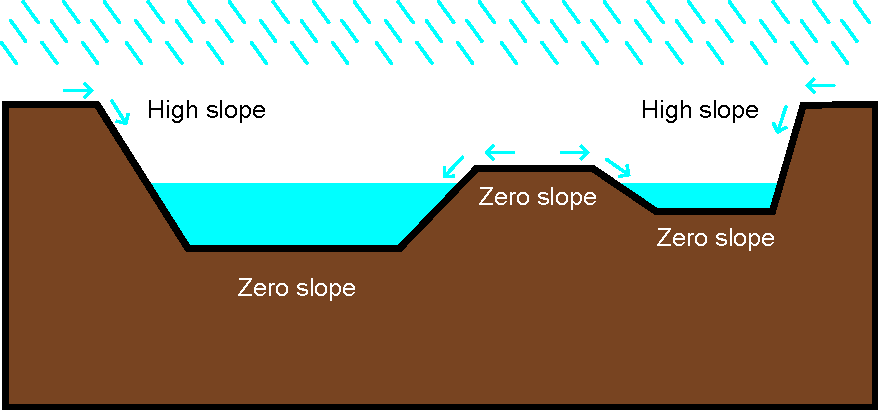
\includegraphics[width=0.9\linewidth]{Chapters/6-Flood/figs/chuva.pdf}
  \caption{Water flows on different slopes terrain.}\label{fig:water_flow}
\end{figure}

Having modelled both types of data, we are able to compute how vulnerable a zone is regarding a rain flood event by combining its elevation and slope. As aforementioned, high elevation reduces (heavy) rain flood risk while lower elevation rises it. In addition, high gradient slopes reduce rain flood vulnerability. The computation of the rain-flood risk $H$ of a zone $z$, defined as $H(z)$, is performed as described in Equation~\ref{eq:flood_risk}.

\begin{equation}
  \label{eq:flood_risk}
  H(z) = \cfrac{1}{e^{\widehat{h}(z) + s(z)}} 
\end{equation}

In this computation, the elevations of the zones are normalised in the range $[-1,~1]$. In fact, the rain flood risk of a zone is relative to the other zones within the AoI, and thus its meaning is constrained to this defined area. Thus, the average elevation zone will get a value of $\widehat{h} = 0$, while the lower zone will be $\widehat{h} = -1$ and the higher zone will be $\widehat{h} = 1$. In this range, the average elevation zone $z_{avg}$ will be $e^{\widehat{h}(z_{avg})} = 1$, being the reference value for elevation parameters.

The slope gradient is the highest ratio of the height differences from the surrounding zones to the zone size ($zl$). Suppose a zone $z_j$ in the vicinity of the zone $z_i$, then the slope gradient is calculated as $\cfrac{|h(z_i) - h(z_j)|}{zl}$. If the zones have the same height, the slope gradient is 0. A difference of height that produces a $45^{\circ}$ angle will return a slope gradient of 1. In this sense, flat surfaces will get 0, having no interference in the computation of the rain-flood risk obtained from the elevation data. However, as long as the gradient slope rises, it will reduce the rain-flood risk computed from the elevation data. This is due to the fact that although a zone may have a lower altitude, water will not accumulate if it flows down due to the gradient slope~\cite{elevation1}.

%2
\subsection{Fluvial data: river-flood risk}

Another relevant parameter for flood risk assessment is the presence of rivers within the AoI. In some situations, it is common that a river crossing a city rises high enough (usually due to heavy rain) and floods its surroundings, which demands the authorities to properly account for that when pursuing flooding resilience. In the presence of a river, it is important to account this factor in the computation of the unified flood risk assessment of the zones, since this factor is expected to increase the overall flood risk.

The first considered element for this particular assessment is the distance from the the river. For each zone within the AoI, it is calculated its distance to the nearest river, since it will have the most significant impact on it. This distance is relevant because the closer a zone is to that river, the higher is its exposure to a river-originated flooding. Actually, the work in~\cite{distance1} shows that even at a distance of 100m from a river, that location is still prone to get flooded by it, thus needing to be properly considered.

Actually, not all rivers are the same. Some rivers may dangerously rise during heavy rains, while some do not even rise at all. This way, a river flood exposure assessment equation can not use the distance from the river as a unique parameter, since the historical flooding behaviour of the river must also be accounted. In this sense, a core element that our approach makes use is the river flooding history, denoted as ``flood quota''. This element indicates the highest historical flood elevation of the river, \textit{i.e}, how high that river have risen in the past. For example, Seine river in Paris has a historical flood elevation of 8.80m (occurred in 1658)~\cite{flood_seine}. In this case, that would be the reference value for flood elevation in our computation for that city. Then, having the historical flood elevation of the river in an AoI, zones lower than that value will probably suffer in the next flood event. Although it does not mean that the river will reach the historical elevation in every next flood event, the history tells that such level has been reached before, thus, it is not an unrealistic concern. Furthermore, even though some rivers have been ``tamed'' by the construction of dams and canals in modern cities, climatic changes are already changing rain precipitation, making hard to predict how the rivers' levels will rise in the near future. With all that said, the highest historical level seems to be a good indication for the intended flood assessment. 

Therefore, the proposed river-flood risk (exposure) computation combines the historical flood quota $q(r)$ of the considered rivers and the normalised distance of the zones from it, achieving a balanced risk parameter that will affect the final assessment of each zone, as shown in Equation~\ref{eq:river_risk_all}.

\begin{equation}
  \label{eq:river_risk_all}
  \begin{split}
    X'(z) = \forall r \in Z_r, 
    \begin{cases}
      \cfrac{1}{e^{\widehat{d}(z, r) \cdot e^4}}    & \quad \text{if } h(z) \leq h(r) + q(r) \\
      0                                             & \quad \text{if } h(z) > h(r) + q(r)
    \end{cases}
  \end{split}
\end{equation}

In order to account the river-flood risk, we identify zones that are affected by a river, processing them separately. This way, the set of all river zones within the limits of the AoI, comprising the subset $Z_r \subset Z$, will support the computation of $X'(z)$, for every zone $r \in Z_r$. Actually, the value of $X'(z)$ is inversely proportional to the normalised distance to the modelled river if the zone elevation $h(z)$ (for a zone outside the river area), is equal or lower than the elevation $h(r)$ (for a zone within the river area), plus the flood quota of that river ($q(r)$). Otherwise, the river-flood risk is 0 for that zone. 

In the occurrence of more than one river within the AoI, the Equation~\ref{eq:river_risk_all} will compute an exposure value for each zone $z$ considering each zone $r$ (over a river), for all rivers. Since different rivers may have different historic flood elevation data, the parameter $q(r)$ will return the historic flood level regarding the river containing the considered zone $r$. Doing so, we provide a flexible mechanism to account the impacts of the rivers in any urban configuration. 

After the performed computations for every zone $z$, the final river-flood risk is performed as presented in Equation~\ref{eq:river_risk}. In this assessment, the considered value is the maximum computed river-flood risk, since we assume the worst-case scenario as the reference.

\begin{equation}
  \label{eq:river_risk}
  X(z) = \max({x, x \in X'(z)})
\end{equation}

%3
\subsection{PoIs data: emergency-response risk}

The flood risk of each zone can also be assessed according to the existing urban emergency mitigation capability, which is accounted by the proximity to response centres (PoIs). When a flood occurs and the local authorities are notified (using phones calls, sensors, or any other means), the typical mitigation procedures begin. First responders like paramedics, firemen, and police agents will move toward the flooded area to take the needed actions. Since time is crucial to reduce victims, these agents need to arrive at their destination as soon as possible. This way, assistance will be provided earlier when affected zones are closer to the PoIs, being then an important factor to decrease the unified flood risk.

Each zone will have an emergency-response risk perception ($E$) based on its distance to every PoI within the AoI. Zones closer to PoIs will have a lower risk perception value than more distant zones. Hence, the risk perception of a zone $z$, here designed by the function $E(z)$, is shown in Equation~\ref{eq:risk_level_ch6}.

\begin{equation}
  \label{eq:risk_level_ch6}
  E(z) = \cfrac{1}{\displaystyle\sum_{j = 1}^{\lvert P \rvert}\left(\cfrac{1}{d^2(z, p_j)} \cdot f(p_j)\right)} 
\end{equation}

The emergency-response risk perception of a zone $z$ is computed taking the inverse of the square distances of that zone to every PoI $p_j$ multiplied by the PoI weight $f(p_j)$, according to the formulations proposed in~\cite{sensorsposition,cityzones}. Then, since this is a risk reducing factor, we take its inverse value. In this equation, the more distant a zone $z$ is from the PoIs, the higher will be its emergency-response risk parameter $E(z)$ (which means it will have a poorer urban service, in average).

\subsection{Flood Risk Assessment}

Having calculated the rain-flood risk (how vulnerable a zone is to heavy rain), river-flood risk (exposure of a zone to a nearby river), and emergency-response risk (how well served a zone is by public services during an emergency), the proposed assessment approach can combine the three parameters to achieve a unified flood risk level for every zone. Figure~\ref{fig:assessment_flow} presents the overall processing flow for that. 

\begin{figure}[ht]
  \centering
  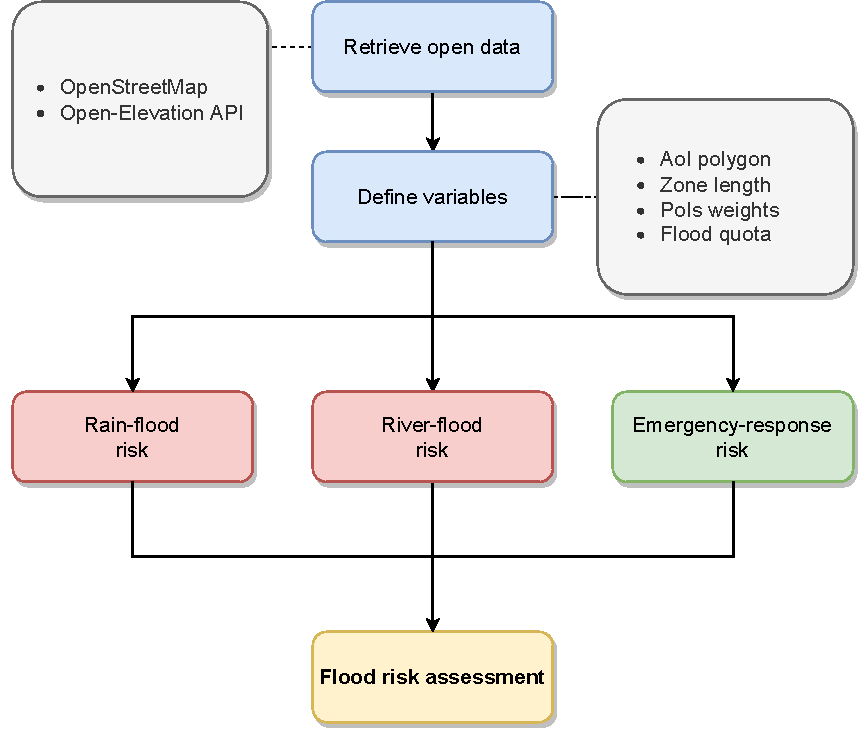
\includegraphics[width=0.9\linewidth]{Chapters/6-Flood/figs/assessment_flow.pdf}
  \caption{Flowchart of the flood risk assessment approach.}\label{fig:assessment_flow}
\end{figure}

The goal of the proposed assessment approach is to provide an overview of urban flood risk, identifying areas (zones) that will be worst affected by flooding, in average, taking open databases as reference. The idea is to numerically evaluate the impact of water accumulation and how the response centres in a city will act to relive eventual conditions. In this sense, a unified flood risk level can be exploited to produce useful heatmaps from the combination of elevation, river zones, and PoIs localisation. Equation~\ref{eq:overall_risk} defines how to compute the unified risk level of each zone, $R(z)$.

\begin{equation}
  \label{eq:overall_risk}
  R(z) = H(z) \cdot \widehat{E}(z) + X(z)
\end{equation}

From Equation~\ref{eq:overall_risk}, the unified flood risk of a zone $z$ will be denoted by its rain-flood risk $H(z)$, that can be relieved by the presence of response centres computed in its risk perception $E(z)$. In any case, the presence of a river will increase the zone flood risk by summing the river-flood exposure $X(z)$. Since not every city has a river, the value of $X(z)$ may be 0 in that case, having no influence in the unified flood risk of the zones.

Actually, Equation~\ref{eq:overall_risk} also demonstrates a generalist approach that allows several layers containing other parameters that are valuable to an assessment process. For example, we added the rain-flood risk $H(z)$ by multiplying it to the emergency-response risk $E(z)$, but other formulations could be proposed. In fact, we expect a ``plugabble'' effect, making it easy to implement other assessment procedures and mixing them together to achieve an overall picture of the risk zones of an AoI, depending on the expected risk modelling.

After computing the unified flood risk of each zone, our approach classifies each zone in one of a group of pre-defined classes. The number of classes is parameterised and is denoted by $M$, \textit{i.e}, if $M = 3$ the classification model will set each zone a risk class ranging from 1 to 3 (low, medium, and high risks, with 3 being the riskiest). Equation~\ref{eq:rc_class} describes the risk class computation of a zone, which adopts a natural logarithmic behaviour for the risk classification since it is very reasonable for urban planning~\cite{log2,log3}.

\begin{equation}
  \label{eq:rc_class}
  C(z) = M - \min\left(M - 1, \left| \left\lceil \ln{R(z)} \right\rceil \right| \right)
\end{equation}

The value of $C(z) = 1$ means that the zone has the best risk level among the zones within the AoI, \textit{i.e}, this zone is not very vulnerable to a rain flood, it is near several PoIs (making it faster to initiate an emergency mitigation procedure), and it has little exposure to river floods. The worst case is when $C(z) = M$, which means that the zone $z$ has the highest risk to rain flood, the poorest positioning regarding the distance and localisation of the PoIs, and very high exposure to a river flood. Intermediate values will be obtained in situations that one bad parameter may be relieved by a good parameter. Once again, it is important to remark that the class of a zone is relative to the defined AoI area due to the employed normalisation process, being pointless to make comparisons among different Areas of Interest.

Figure~\ref{fig:zones_and_pois_classified} demonstrates a visual example of the risk class computation.

\begin{figure}[ht]
  \centering
  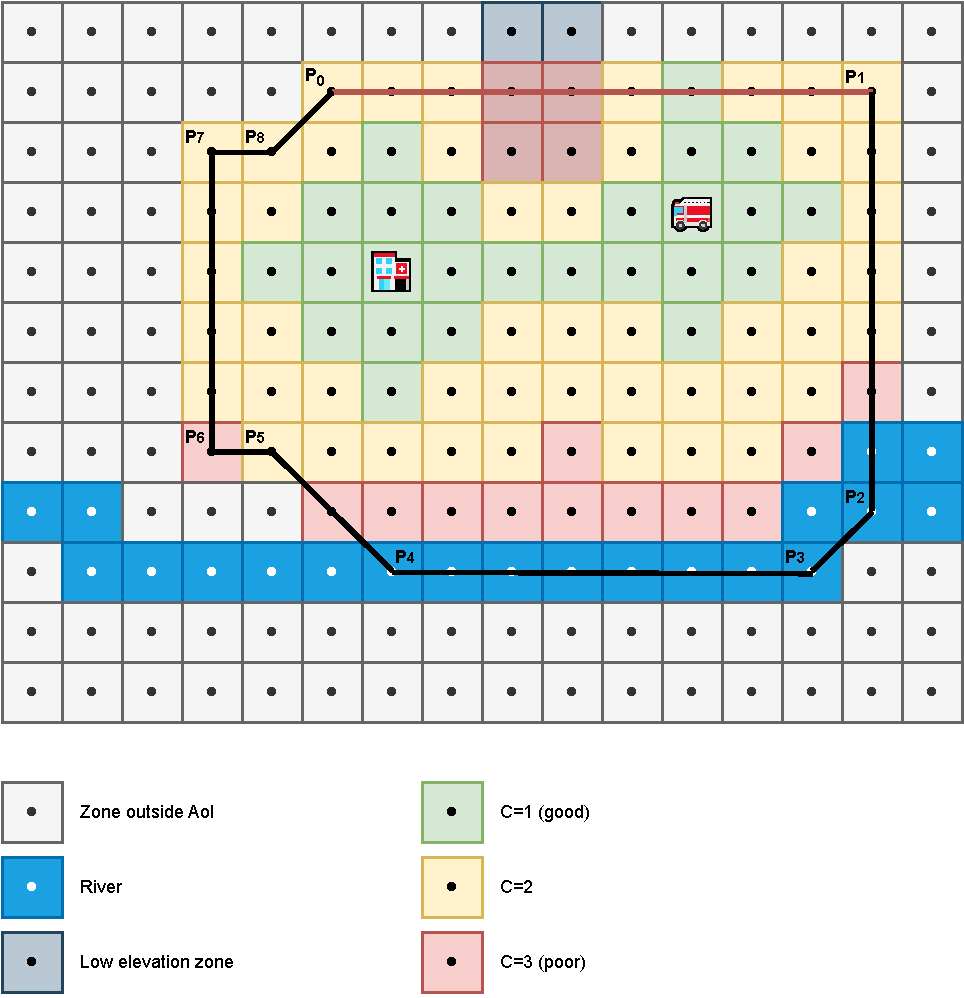
\includegraphics[width=0.9\linewidth]{Chapters/6-Flood/figs/zones_and_pois_classified.pdf}
  \caption{Risk classification of the zones based on the combined processing of rain-flood risk, rain-flood risk, and emergency-response risk.}\label{fig:zones_and_pois_classified}
\end{figure}

%%%%%%%%%%%%%%%%%%%%%%%%%%%%%%%%%%%%%%%%%%
\section{Experiments and achieved results}\label{sec:simulation_ch6}

Porto, a historic city situated along the banks of the Douro River in northern Portugal, was chosen as the target city for the evaluation of our proposed approach. It is the second-largest city in Portugal, renowned for its cultural heritage, vibrant atmosphere, and economic significance. However, its geographical location near the Douro River places it at risk of flood events, making it an ideal case for flood risk assessment.

The city of Porto holds a special place in the context of flood risk assessment due to its historical and contemporary susceptibility to river flood. The Douro River, which flows through Porto before reaching the Atlantic Ocean, has been the site of recurrent flood events over the centuries. Historical flood data for the Douro River in Porto provides a rich repository of information on past flood events, their extent, and the resulting damage. These events have left an indelible mark on the city's infrastructure and inhabitants.

The highest flood elevation in the history of Douro River along the city of Porto was 26.3m in 1909~\cite{inundacaodouro}, thus, this was the considered value in Equation~\ref{eq:river_risk}. The AoI was delimited to the boundaries of the city and the retrieved PoIs were fire brigades, police stations, and hospitals. 

At this point, an important remark is the proper selection of relevance weights for the PoIs. Usually, firefighters and police agents are the first responders that act in mitigation processes when a river flood occurs in Portugal, while hospitals are used to provide medical assistance to the victims and also as a hub to dispatch and receive incoming ambulances. Although ambulances and hospital services are requested in a flood event, firefighters may be perceived as the most important responders in such mitigation scenario, followed by police agents. But the other way around is also a reasonable choice, with police agents being more relevant depending on the cities' characteristics and emergency strategies. In this sense, in order to define a reference for the experiments, the weight for fire brigades was empirically set to 10 and the weight for police stations was set to 5, while hospitals were set to 4, meaning that fire brigades were twice more important than police stations which, in turn, were slightly more relevant than hospitals in our experiments. Although we defined those weights, different values could be used in the same approach since our proposal does not define fixed weights for any PoI. 

The algorithms were executed on a computer with a 6-core AMD Ryzen~5~4600H 3.0~GHz processor, 16~GB of RAM, running Debian~GNU/Linux 12. All the code was implemented using the Python~3.11 language, making use of the MultiProcessing library.

Figure~\ref{fig:porto_elevation} presents the elevation of every zone within the defined AoI, created using the Open-Elevation API, for zones with $zl = 90m$. As expected, the elevation of zones near the coast and banks of the Douro River is lower, being potentially more affected by water accumulation during a flood.

\begin{figure}[ht]
  \centering
  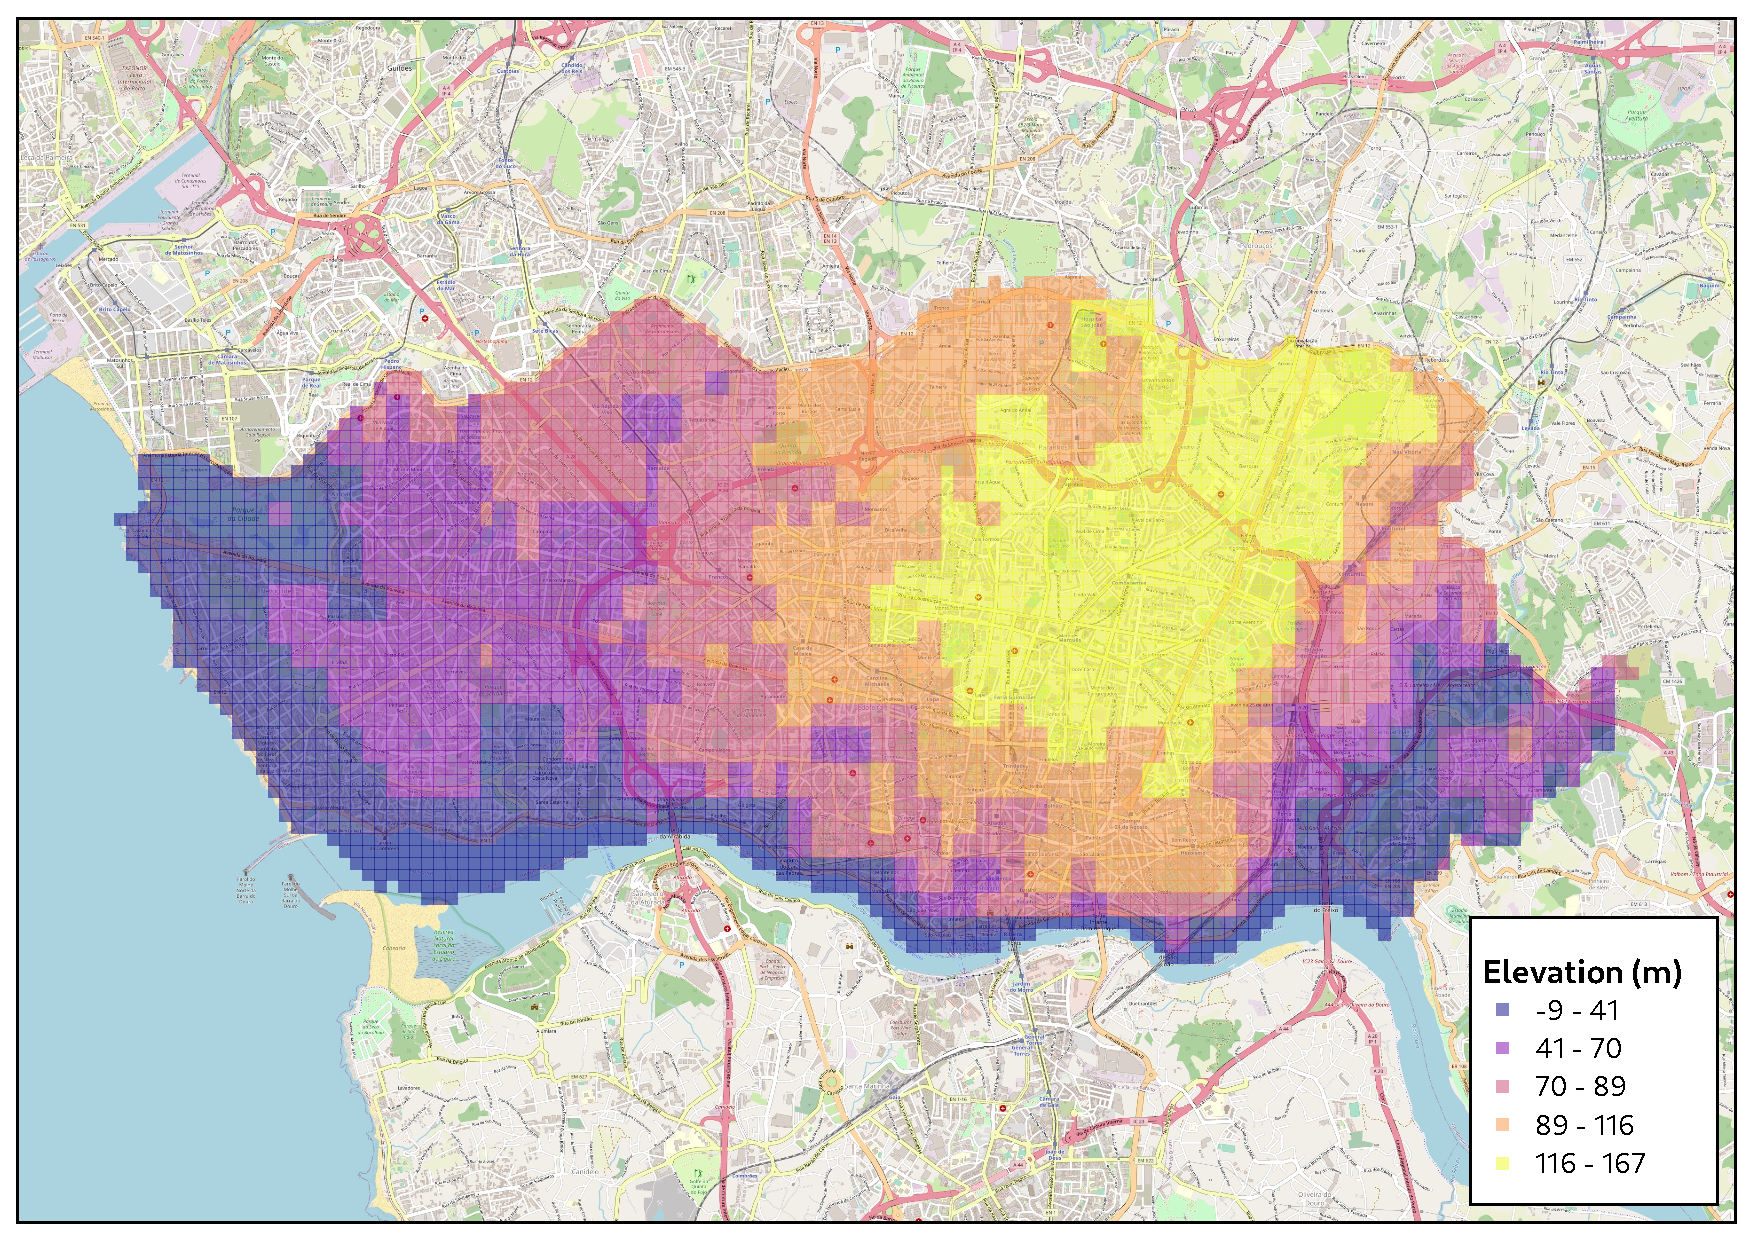
\includegraphics[width=0.9\linewidth]{Chapters/6-Flood/figs/porto_elevation.pdf}
  \caption{Elevation data for Porto.}\label{fig:porto_elevation}
\end{figure}

The retrieved list of PoIs within the defined AoI is depicted in Figure~\ref{fig:poisporto}. The colour of the dots represents the PoI type in our experiments. 

\begin{figure}[ht]
  \centering
  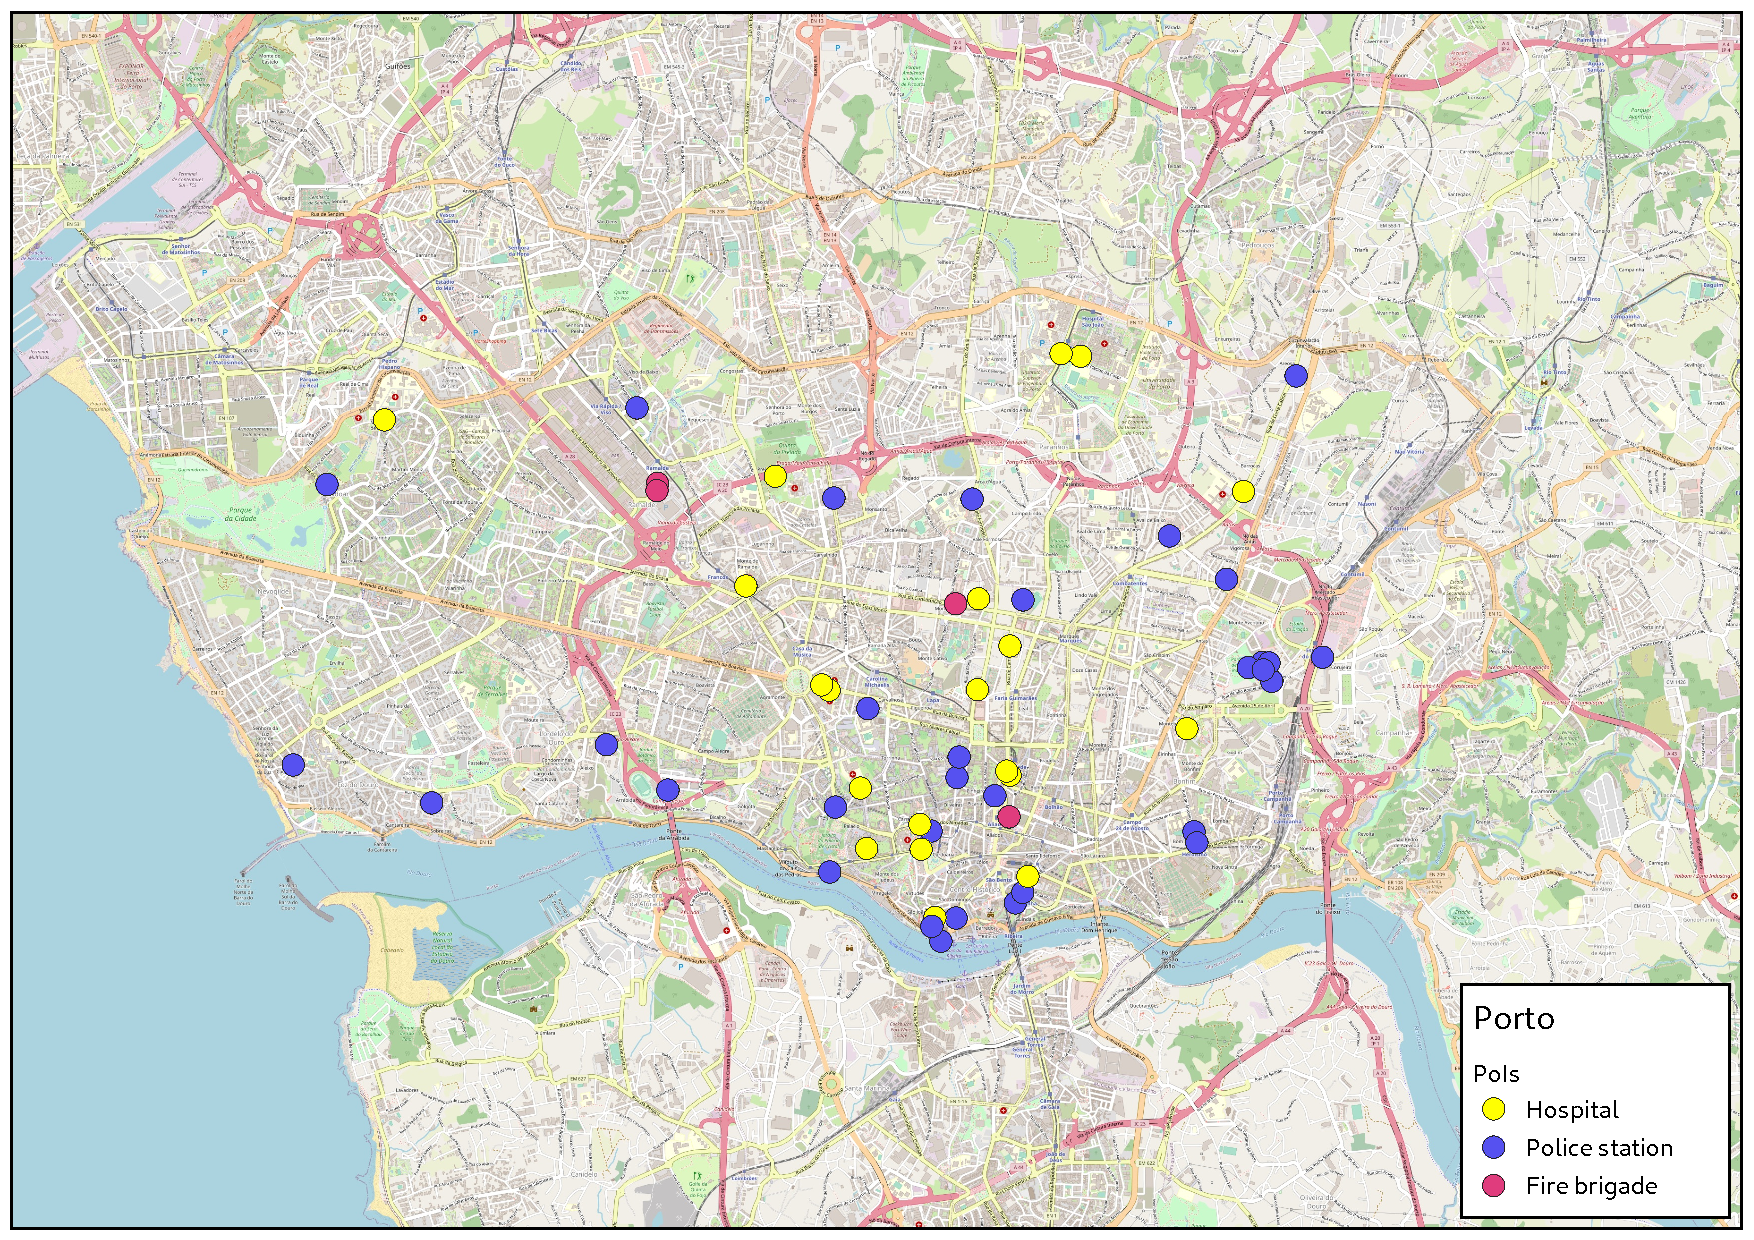
\includegraphics[width=0.9\linewidth]{Chapters/6-Flood/figs/porto_pois.pdf}
  \caption{Emergency-response centres in Porto.}\label{fig:poisporto}
\end{figure}

Figure~\ref{fig:porto} shows the final flood risk classification for the city of Porto, combining the three computed risk parameters. In that Figure, zones with lower risk are classified as $C=1$ (green), while the riskiest zones have $C=3$ (red).

\begin{figure}[h!]
  \centering
  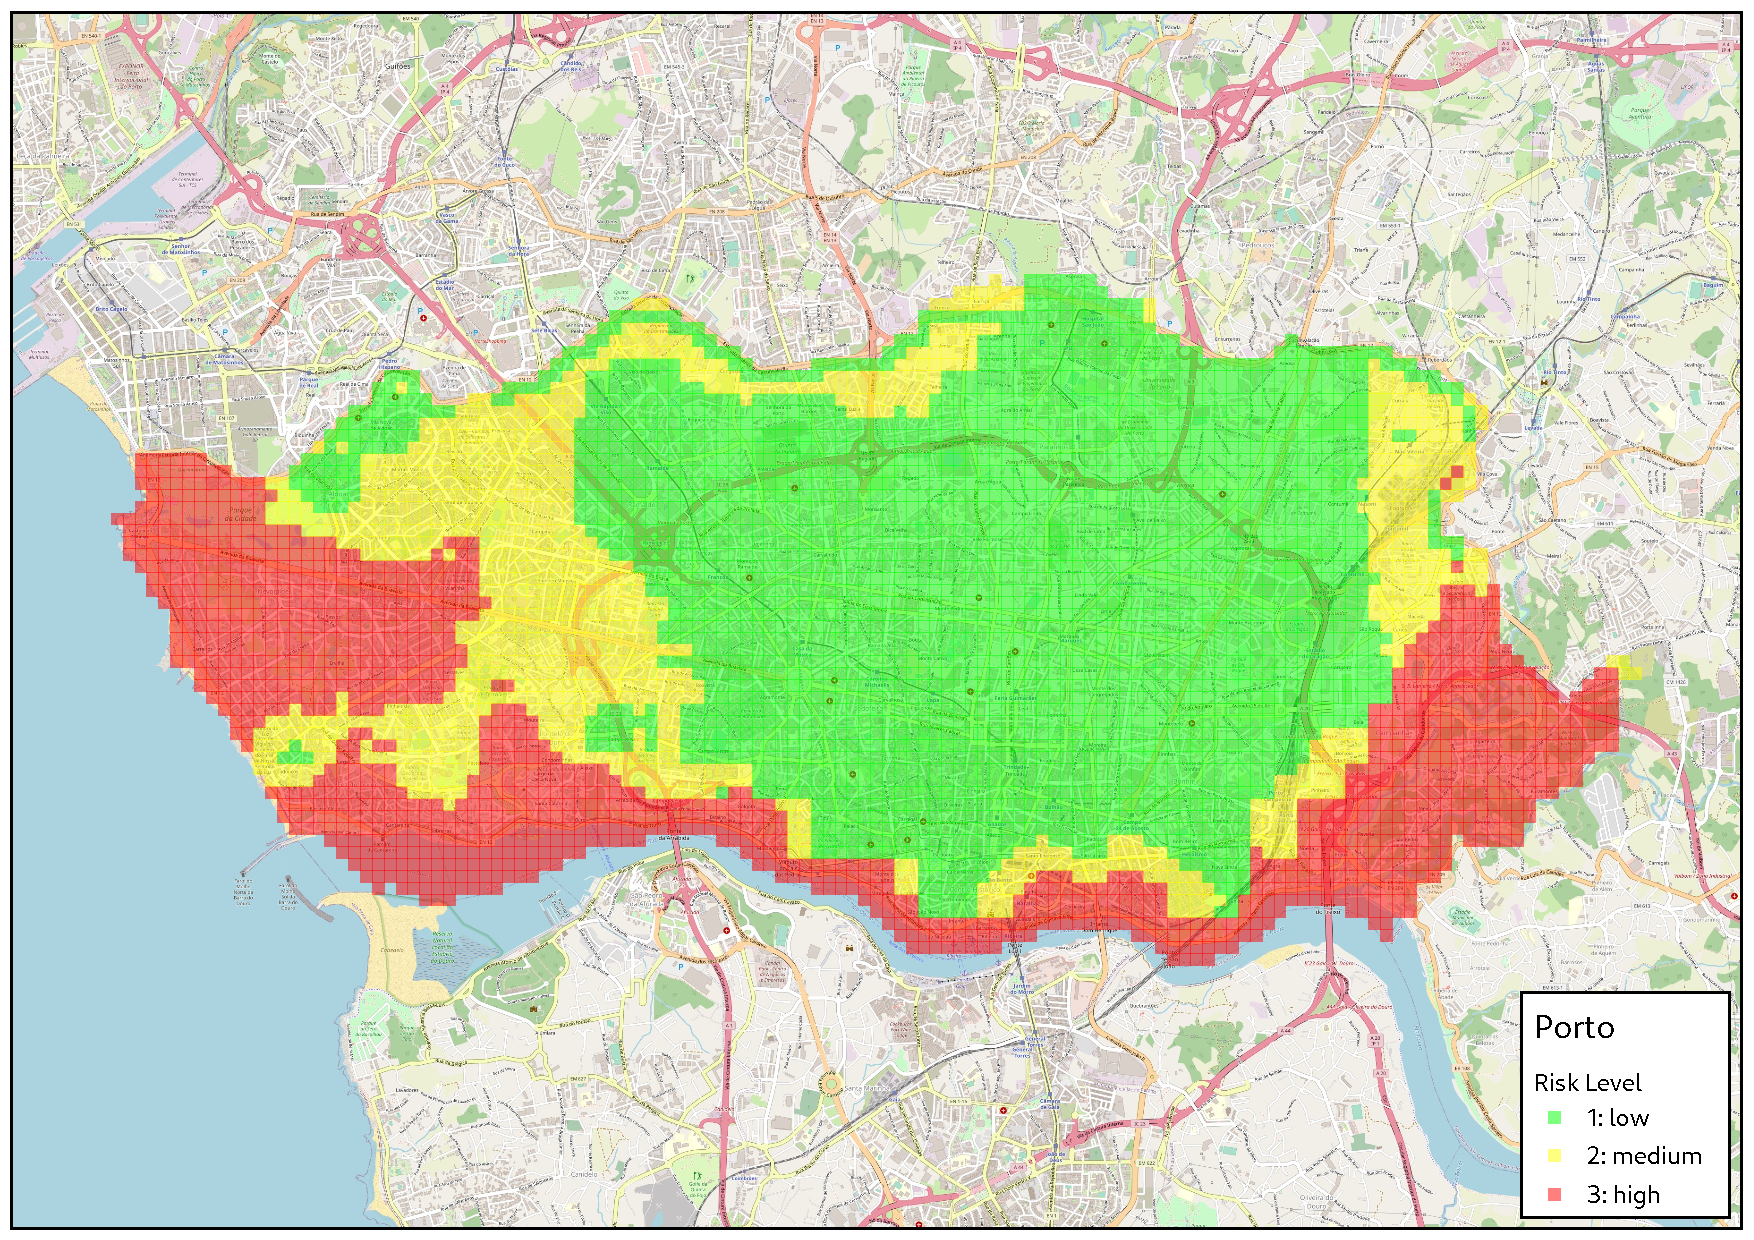
\includegraphics[width=0.9\linewidth]{Chapters/6-Flood/figs/porto.pdf}
  \caption{Flood risk classification for Porto.}\label{fig:porto}
\end{figure}

In order to get a bigger picture of the flood risk assessment in the surroundings of the Douro River we have applied our approach in a broader area comprising not only the city of Porto, but also part of its metropolitan area covering both banks of the river. Figure~\ref{fig:porto_gaia_elevation} shows the elevation levels for the computed zones in a rectangular AoI (cities of Porto and Vila Nova de Gaia).

\begin{figure}[ht]
  \centering
  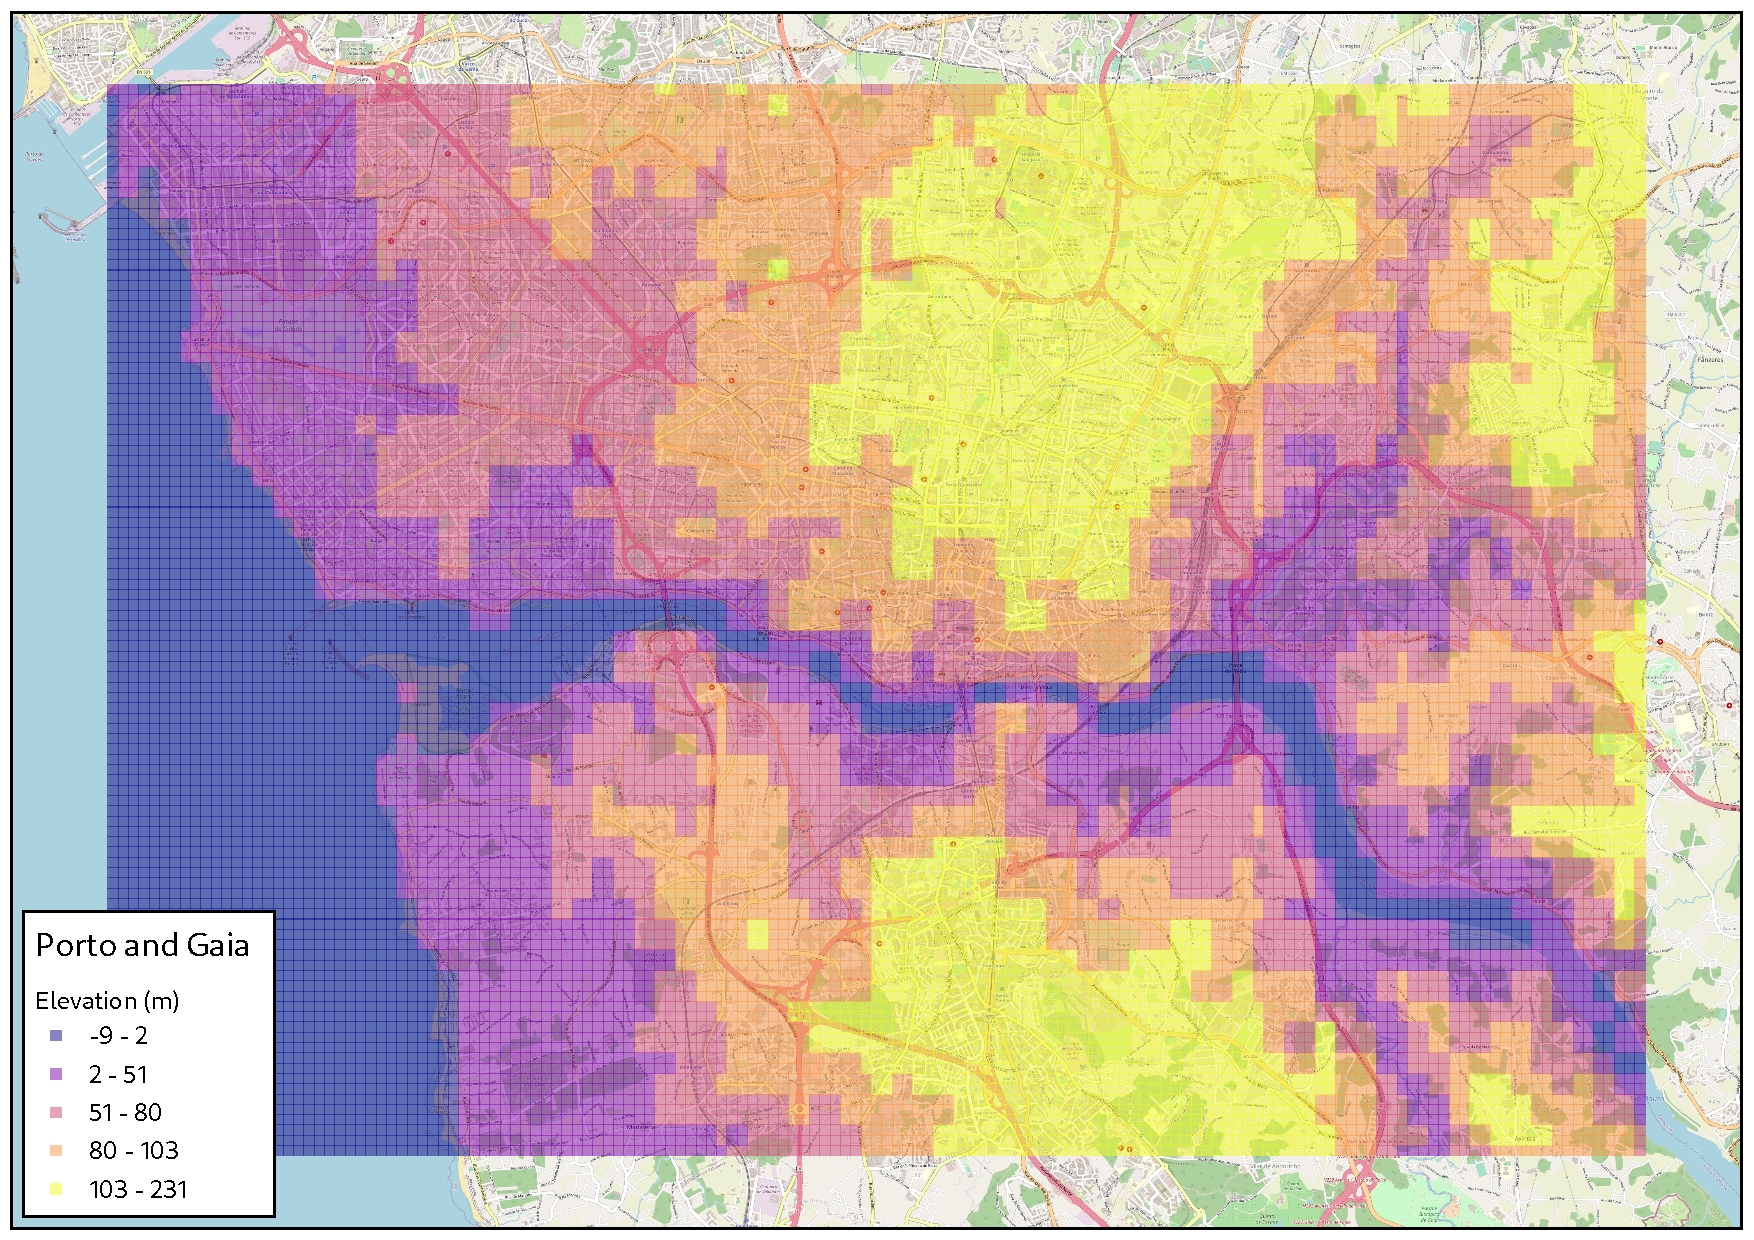
\includegraphics[width=0.9\linewidth]{Chapters/6-Flood/figs/porto_gaia_elevation.pdf}
  \caption{Elevation data for Porto and Vila Nova de Gaia.}\label{fig:porto_gaia_elevation}
\end{figure}

Having all risk parameters for this new AoI, we applied the proposed assessment approach to achieve the desired flood risk classes, as depicted in Figure~\ref{fig:porto_gaia}. 

\begin{figure}[ht]
  \centering
  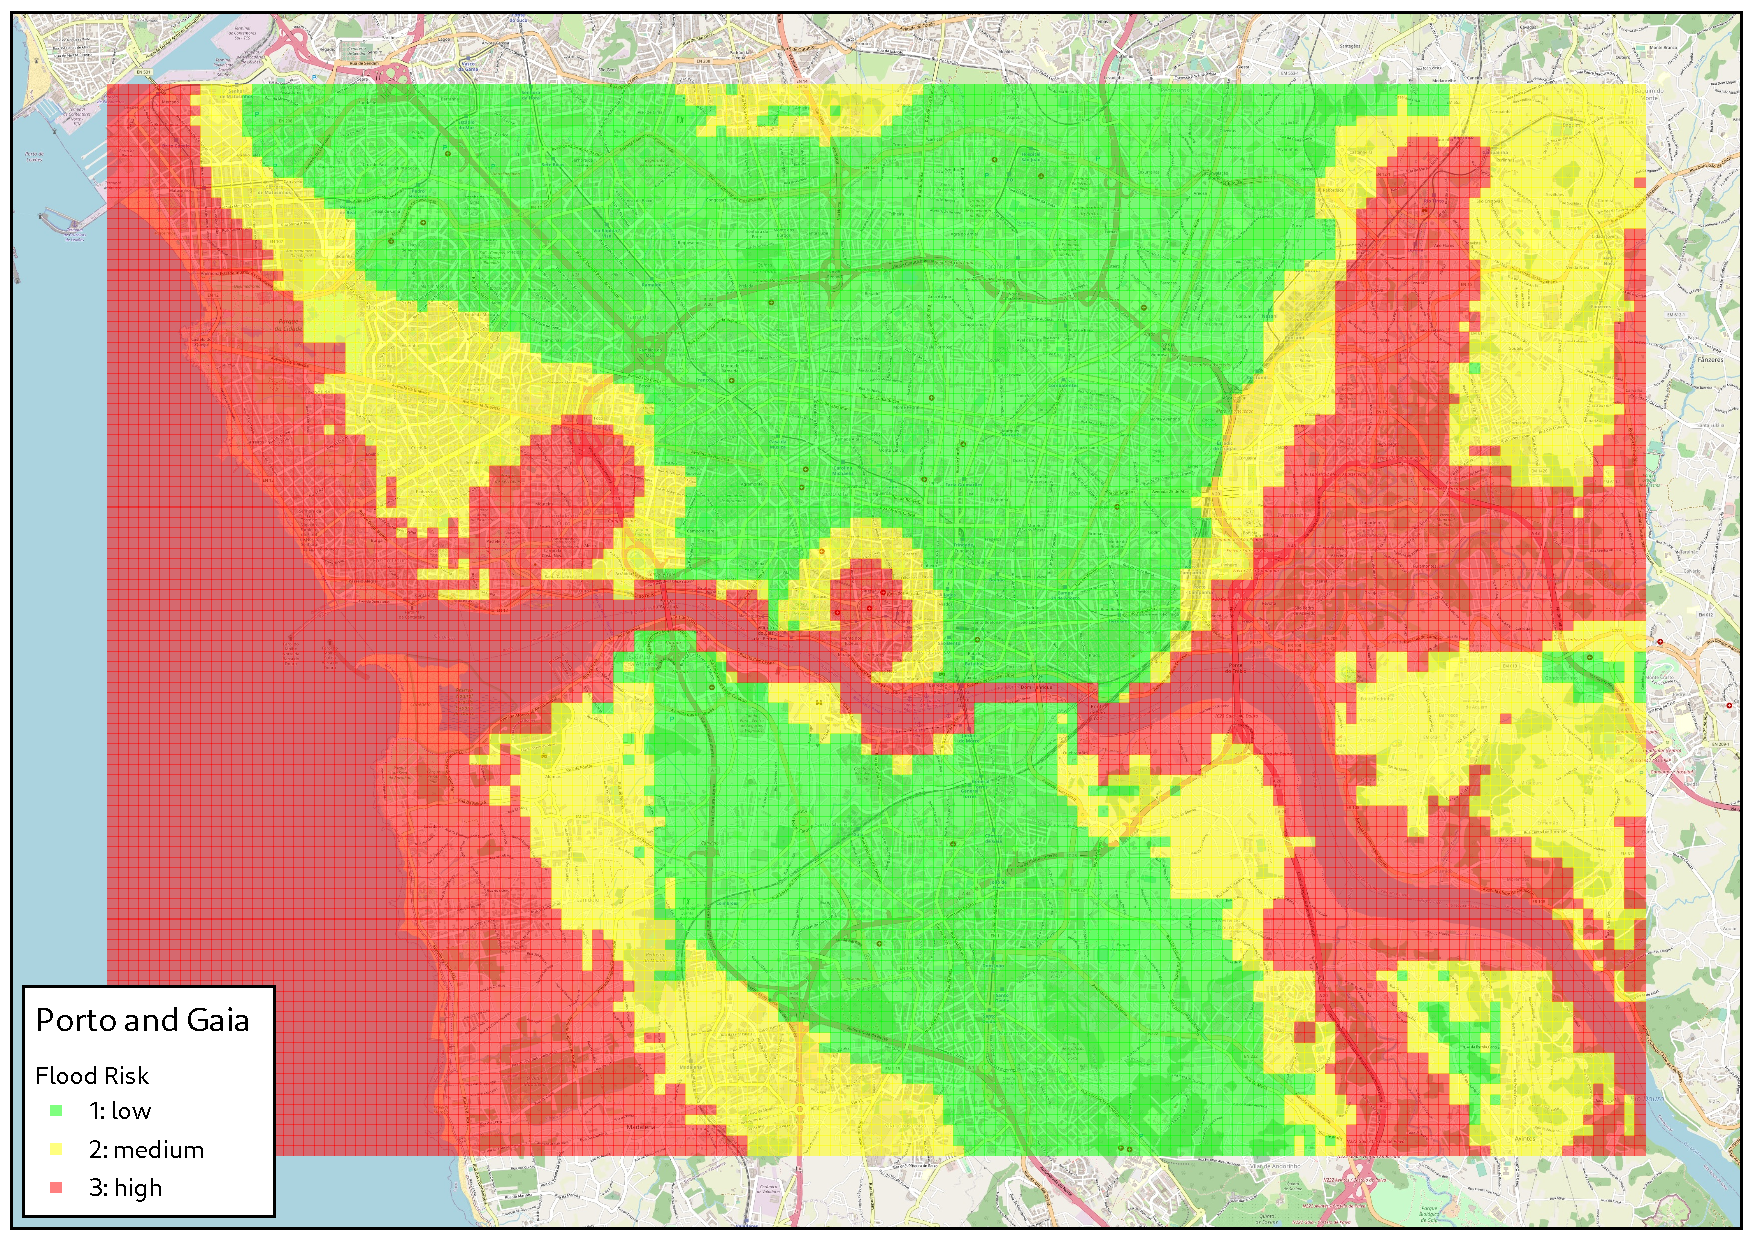
\includegraphics[width=0.9\linewidth]{Chapters/6-Flood/figs/porto_gaia.pdf}
  \caption{Flood risk classification for Porto and Vila Nova de Gaia.}\label{fig:porto_gaia}
\end{figure}

At a first glance, one may notice that the assessment for the area of Porto differs in both scenarios. This happens because the proposed assessment approach provides a relative classification, \textit{i.e}, the three different classification levels mark the zones with low or high risk relative to each other, and within the defined AoI. In this sense, red zones are riskier than yellow and green zones in the considered context: If the AoI changes, the resultant assessment and risk classification may change too.

Finally, after the performed computations, we could see that the intended flood risk assessment could be satisfactorily performed as expected. Since open databases are used as reference, the only concern was to find the worse historical flood record for the Douro river, which is easy to be discovered (or even loosely estimated). Therefore, we believe that the proposed approach could be easily adopted as a practical tool when improving urban resilience.

%%%%%%%%%%%%%%%%%%%%%%%%%%%%%%%%%%%%%%%%%%
\section{Applications and research trends}\label{sec:applications}

The proposed approach is a generalist method that can be applied to any city in the world without restrictions, contributing to the development of smart city initiates targeted at flooding resilience. The use of open data from OpenStreetMap and Open-Elevation API makes that possible, as well as the defined comprehensive mathematical model. Thus, we expect that our approach would allow for several applications in the smart cities landscape, particularly regarding emergency detection, alerting, and mitigation, with a lot of potential significant results.

Some of the possible applications leveraging the proposed flood risk assessment approach is the deployment planning of sensing units. The work in~\cite{positioning} exploited only the existence of PoIs when detecting any kind of urban emergency, and we believe that similar results could be achieved when also considering flooding. In this case, the classification of the zones would guide the distribution of a previously defined set of sensing units, particularly created to detect flood-related emergencies~\cite{floodhardware1,floodhardware2}. Although it might seem obvious that water sensors must be positioned on the river areas, the performed flood risk assessment may indicate the most exposed zones, aiding the planning of sensors deployment by depicting which areas are most exposed.

In a similar trend, the deployed sensors could be combined with the computed risk maps when finding escape routes during a flooding, guiding people through less risk zones. This could avoid the trapping of evacuees in flooded areas, which could have potentially dangerous outcomes~\cite{rescuing2,rescuing3}. For that, mobile applications could be developed to leverage interactive heatmaps, allowing users to explore different areas of the city and understanding the varying levels of flood risk. Users could receive notifications and alerts based on their location within the heatmap.

Urban planning can also be benefited. In a dense urban area, heavy rain flood is a real risk and must be tackled to prevent damages to the city infrastructure and its inhabitants~\cite{rainflood}. In this sense, the rain flood risk classification will reveal zones that are more geographically vulnerable. This assessment may reveal areas in a city that may require a suitable drainage infrastructure that is capable of draining all the water from a heavy rain, avoiding flood-related disasters.

In the overall picture, the proposed flood risk assessment may aid public authorities in better planning the infrastructure of a city, discovering more vulnerable and exposed areas that need special equipment to detect, alert, and mitigate flooding events, preventing excessive losses and damages due to an unprepared urban setting. When concerning existing tools, the proposed approach could also be incorporated, improving their achieved results. By implementing the rain-flood and river-flood risks assessments, tools like CityZones~\cite{cityzones} could be enhanced to provide better results for flood risk classification, and similar results are expected for other tools devoted for risks assessment.

Our proposed assessment approach could also be integrated within the context of a smart city, particularly in the scenario of multi-systems interfacing~\cite{survey}. When integrating flood risk heatmaps with smart infrastructure, urban systems can exploit risk data for optimisations. For example, smart traffic lights can be used to avoid that vehicles move toward flooded areas~\cite{traffic1,traffic2}, which could bring danger to the drivers or even compromise the rescuing of affected people due to unwanted traffic. During a heavy rain, riskier areas could be already considered for this processing, reducing traffic even before a flood emergency is raised.

Finally, by applying our proposed approach to the city of Porto, we could leverage georeferenced data to assess and potentially enhance the city's flood resilience in the face of future challenges. As smart cities continue to evolve, managing and mitigating flood risks becomes a crucial aspect of urban planning and development. Porto's experience with the Douro River floods offers invaluable insights for not only safeguarding its future but also providing a blueprint for other urban areas facing similar challenges. We believe that the development of data-driven methodologies to assess risk levels in cities can aid authorities to better plan the growing of urban areas and the building of new response centres in order to prevent or, at least, reduce life and economic losses, reinforcing the applicability of our approach.

%%%%%%%%%%%%%%%%%%%%%%%%%%%%%%%%%%%%%%%%%%
\section{Conclusions}\label{sec:conclusion_ch6}

Among the many types of emergency events that may happen in an urban area, flood is the most recurrent and the one which makes more impact in a city. In order to prepare a smart city for such events, a risk classification mechanism must be used to identify the flood prone areas and allow for better response and preparedness. In this sense, this article proposed a flood risk assessment methodology that makes use of open data as reference, making it generic and very adaptive. The performed experiments for the city of Porto, Portugal, presented some promising results.

The river geolocalisation data obtained from OpenStreetMap allows us to compute the river-flood risk regarding the proximity to river zones. Taking open elevation data from Open-Elevation API, it is possible to calculate the slope of each zone and combine all these data to also compute rain-flood risk, selecting regions that are too low and surrounded by high slope zones. The elevation data is also used in the river-flood risk assessment to verify which zones in the river surroundings could benefit from an elevation difference higher than the historical flooding heights. Finally, emergency-response data from OpenStreetMap is also accounted. This combined approach has shown that open and publicly available data are valuable for risk assessment, helping the planning and maintenance of emergency infrastructure in an urban area.

As future works, other types of floods will be considered, particularly the ones resulted from tsunamis and rapid snow melting. Several cities in Europe are already being affected by climates changes, making them more prone to flood events~\cite{warming}. Because of these changes, extreme climatic events are predicted to increase in the next years~\cite{warming2}, making cities more prone to tsunamis and coastal flooding. By gathering other types of parameters related to climatic changes, such as snow depth history and temperature changes, we could extend our approach to assess new perspectives of flood risks in cities.

\printbibliography[heading=subbibliography]

\end{refsection}
\selectlanguage{brazil}
